\subsection{The Sensing Subsystem}
This section will look at the integration of LoRa-E5 MCU and the three main atmospheric sensors in the Aether nodal system. The MCU in the Aether node will use I2C communication protocol to communicate with the sensors and gateway module. Each node is equipped with a Sensirion PM sensor, a Renesas ZMOD4510 sensor, and a Bosch BME688 sensor. The particulate matter sensor is capable of detecting both particulate matter 2.5 PM2.5, and particulate matter 10 (PM10). Renesas' ZMOD4510 sensor is equipped with non-selective nitrogen dioxide (NO2) measurement capabilities with a selective measurement of ozone (O3) as well. The Bosch BME sensor gives the Aether node the flexibility to measure multiple types of gases including Volatile Organic Compounds (VOCs), volatile sulfur compounds (VSCs) and other gases such as carbon monoxide and hydrogen in addition to pressure, temperature & humidity sensor through AI and machine learning models. The MCU will be connected to an antenna on the outside of the enclosure to communicate through the LoRa-WAN network.

\subsubsection{Bosch BME688 Sensor}
The Bosch BME688 detects Volatile Organic Compounds (VOCs) and Volatile Sulfur Compounds (VSCs) and other gases through the use of sophisticated AI embedded in the system and machine learning algorithms. This sensor comes in a 3.0 mm x 3.0 mm x 0.93 mm metal lid 8-pin LGA. Aether's Bosch BME688 sensor supports two digital communication interfaces: I2C and SPI. As previously discussed, I2C will be the main source of communication in our overall design and the BME688 I2C interface can support the Standard, Fast and High Speed modes of the sensor. To activate the I2C interface on the Bosch sensor, the VDDIO pin 6 is connected the chip select status (CSB) pin 2. To power the sensor, VDD pin 8 is connected to the 3.3V power rail and tothe VDDIO pin. Both VDD and VDDIO are paired with decoupling capacitors connected to ground to help oppose fast changes of voltage. The pins dedicated to the I2C communication interface are serial clock (SCL), data (SDA), and slave address LSB (SDO). Because SDI is bi-directional, it is connected to VDDIO via a pull-up resistor. Once the I2C communication interface is activated on the chip, the next step is to make the appropriate connections to the LoRa microcontroller. The serial data input (SDI) pin 3 is directly connected to the serial data (SDA) pin 6 on the microcontroller. The serial clock (SCL) pin on the Bosch sensor is connected to pin 5 on the microcontroller. The SDO pin on the sensor is tied to ground for the default slave address.  
\paragraph{}

\subsubsection{Renesas ZMOD4510 Sensor}
The ZMOD4510 is a 12-pin LGA assembly with dimensions of 3.0 ×3.0 ×0.7mm equipped with an I2C communication protocol. This is the sensor responsible for detecting nitrogen dioxide and ozone in the the Aether node. The serial clock and serial data pins for the I2C interface on the sensor module will go connected to the respective pins on the LoRa microcontroller, pins 5 and 6. VDD is the voltage supply for the ZMOD4510 and VDDH is the voltage supply for the integrated heater in the ZMOD4510. The VDDIO pin is the voltage supply for I/O-interface in ZMOD4510. These 3 voltage supply pins will all be connected to the 3.3V power rail. Pin 3 on the ZMOD4510 is the interrupt pin on the sensor. This pin will read HIGH when a measurement is running and LOW when a measurement has finished. It will be connected to GPIO pin 11 on the LoRa microcontroller. The VSS pins for the ZOMOD are the sensors ground references and will therefore be tied to ground. The ZMOD is equipped with a RES function on pin 11. This is an  active low pin connected to the 3.3V power rail via a 10KOhm pull-up resistor. 

\subsubsection{Sensirion Particulate Matter Sensor}
Aether's SPS30 sensor will be responsible for collecting particulate matter data for the node. Unlike the other 2 sensors discussed, the SPS30 will not be soldered directly onto the main PCB board. The interface is a 5-pin JST connector located at the side of the sensor opposite to the air inlet/outlet. Because this sensor relies on a built-in fan to collect ambient particle samples, it will be placed at the very edge of the inner housing for the node. A JST female wire harness plug will then be used to connect the sensor to the 5-pin ZHR-5 connector on the main PCB board. SPS30 offers both UART and I2C communication. To activate the I2C communication protocol on the SPS30 sensor, the select (SEL) pin must be tied directly to ground. This particulate matter sensor operates with a 5V input, which is the reason we needed to design a 5V power rail in Aether's power schematic through a boost converter. The VDD pin on the SPS30 is the supply voltage pin that will be powered by this 5V rail. Pins 2 and 3 are the SDA and SCL pins on the SPS30, respectively. The I2C pins will be connected to the respective pins on the LoRa microcontroller and tied to 10kOhm pull-up resistors connected to the 3.3V power rail. A 3.3V input was used instead of 5V for the SDA and SCL pins because the pins are LVTTL 3.3V compatible. Using 3.3V instead of 5V for the I2C pins ensures no over-voltage damage is done to the microcontroller since it operates under the 5V range. The overall schematic design for the Aether node MCU and sensor system can be seen in Figure \ref{fig:MCU_Sensor}

\begin{figure}
    \centering
    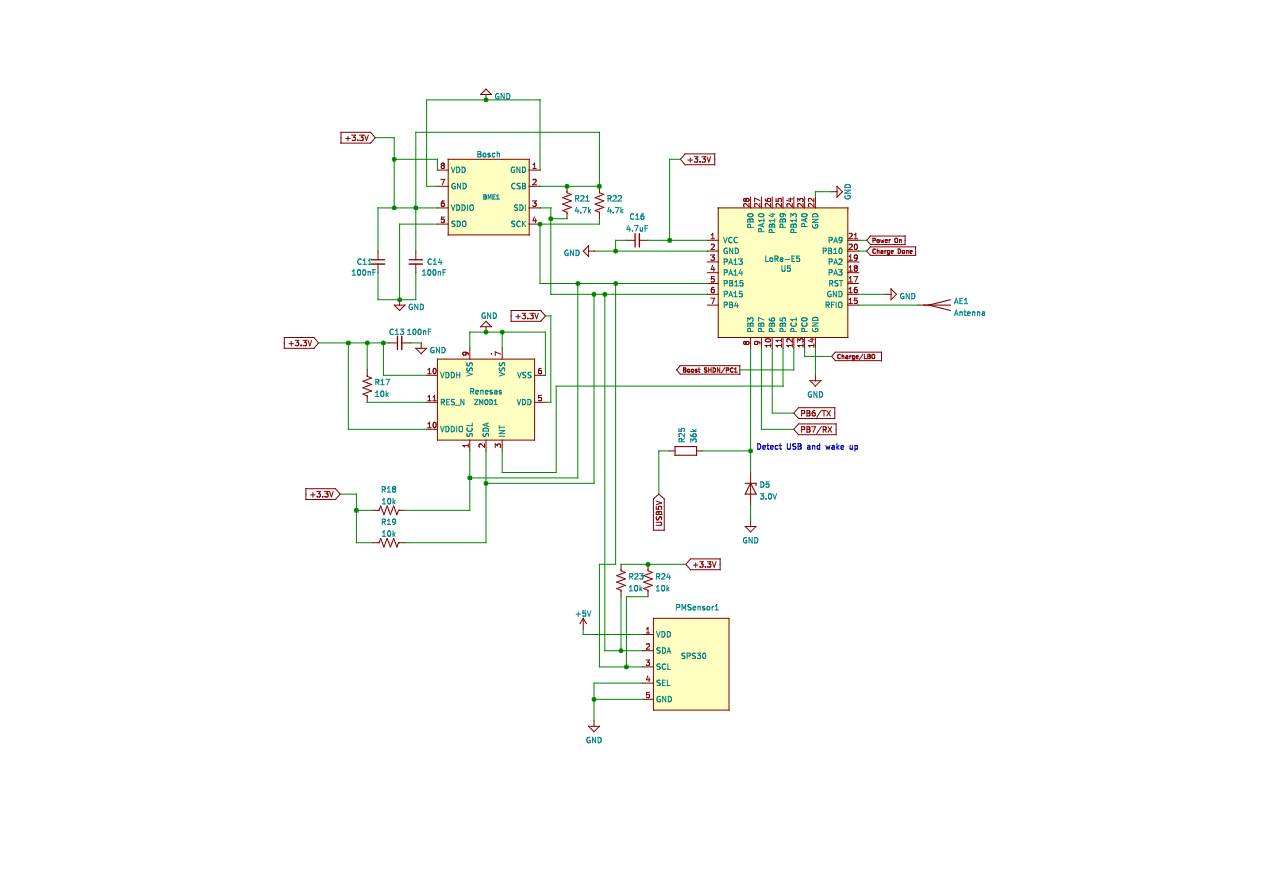
\includegraphics[scale=.75]{figures/MCU_Schematic.jpg}
    \caption{Aether Node MCU and Sensor System Schematic}
    \label{fig:MCU_Sensor} 
\end{figure}
